\documentclass[a4paper,11pt]{ltjsarticle}
\usepackage{geometry}
\geometry{top=25mm,bottom=25mm,left=25mm,right=25mm}
\usepackage{graphicx}
\usepackage{amsmath,amssymb,bm}
\usepackage{hyperref}
\usepackage{float}
\usepackage{caption}
\usepackage{subcaption}
\usepackage{booktabs}
\usepackage{siunitx}
\usepackage{listings}
\usepackage{xcolor}
\usepackage{physics}
\usepackage{microtype}

\hypersetup{
  pdftitle={数理工学実験レポート},
  pdfauthor={中塚一瑳},
  colorlinks=true,
  linkcolor=blue,
  citecolor=blue,
  urlcolor=blue
}

% -------------------------
% ユーザ定義マクロ
% -------------------------
\newcommand{\StudentID}{1029366161}
\newcommand{\AuthorName}{中塚一瑳}
\newcommand{\CourseName}{数理工学実験}
\newcommand{\ChapterTitle}{第3章(最小二乗法)}
\newcommand{\ExperimentDate}{\today}

% 図・表フォルダパス(必要なら変更)
\newcommand{\graphdir}{graphs}

% 数式用の簡易マクロ
\newcommand{\R}{\mathbb{R}}
% \newcommand{\norm}[1]{\left\lVert#1\right\rVert}  % physics パッケージで既に定義済み

% listings 設定(R を例示)
\lstset{
  basicstyle=\ttfamily\footnotesize,
  breaklines=true,
  frame=single,
  numbers=left,
  numberstyle=\tiny,
  language=R,
  keywordstyle=\color{blue},
  commentstyle=\color{gray},
  stringstyle=\color{teal},
  showstringspaces=false
}



% キャプションのフォント調整
\captionsetup{font=small,labelfont=bf}

% -------------------------
% 本文
% -------------------------
\title{数理工学実験レポート\\[4pt]\large \ChapterTitle}
\author{学籍番号 1029366161 \quad 中塚一瑳}
\date{\ExperimentDate}

\begin{document}

\maketitle
\begin{abstract}
% 要旨をここに記述
\end{abstract}

\tableofcontents
\clearpage

% \section*{表記・略記}
% 本レポートにおける表記と略記を示す。必要に応じて編集すること。
% \begin{itemize}
%   \item $\R$:実数全体
%   \item $\|\cdot\|$:ユークリッドノルム(明示が必要な場合は添字を用いる)
%   \item 各種パラメータや記号は本文中で定義する
% \end{itemize}

% ===== 例:実験テンプレート =====
\section{はじめに}
本実験第2回では,最小二乗法の基礎とその実装手法を学ぶことを目的とする。具体的には,観測データからのパラメータ推定,重み付き・逐次最小二乗法,データ分割・推定値の合成を通して,推定精度と計算効率の違いを実験的に比較する。


\section{最小二乗法とその評価方法}

\subsection{原理・方法}

観測モデルを
\begin{align}
 y_i = f(\theta, x_i) + w_i
\end{align}
とする.加法雑音 $w_i$ は平均 $0$,観測ごとに独立,同一分布であり,共分散は有限と仮定する.
ここでは $f(\theta, x) = \phi(x)\theta$ としてパラメータに対して線形とし,最小二乗問題
\begin{align}
 \min_{\theta}\sum_{i=1}^{N}\lVert y_i - \phi(x_i)\theta\rVert^2
\end{align}
を解く.解は
\begin{align}
 \hat{\theta}_N
  = \Big( \sum_{i=1}^{N} \phi_i^\top \phi_i \Big)^{-1}
    \sum_{i=1}^{N} \phi_i^\top y_i,
 \qquad \phi_i := \phi(x_i).
\end{align}

また雑音分散が未知の場合の推定量および推定誤差共分散は
\begin{align}
 \hat{\sigma}^2
 &= \frac{1}{N-n} \sum_{i=1}^{N} \lVert y_i - \phi_i \hat{\theta}_N \rVert^2, \\
 \widehat{\mathrm{Cov}}(\hat{\theta}_N)
 &= \hat{\sigma}^2 \Big( \sum_{i=1}^{N} \phi_i^\top \phi_i \Big)^{-1}
\end{align}
で与えられる.

当てはまりの評価には決定係数
\begin{align}
 C = \frac{\sum_{i=1}^{N}\lVert \phi_i \hat{\theta}_N - \bar{y} \rVert^2}
          {\sum_{i=1}^{N}\lVert y_i - \bar{y} \rVert^2},
 \qquad
 \bar{y} = \frac{1}{N}\sum_{i=1}^{N} y_i
\end{align}
を用いる.以上は資料3.2の線形最小二乗および評価に対応する.


本実験では $\phi(x)$ として設計した特徴量から行列
\begin{align}
 X = \begin{bmatrix}
  \phi(x_1)^\top \\
  \vdots \\
  \phi(x_N)^\top
 \end{bmatrix}
\end{align}
を構成し,観測データを
\begin{align}
 y = [y_1; \dots; y_N]
\end{align}
として用いる.パラメータ推定量は
\begin{align}
 \hat{\theta} = (X^\top X)^{-1} X^\top y
\end{align}
で与えられる.

残差は
\begin{align}
 r = y - X\hat{\theta}
\end{align}
とし,雑音分散推定量は
\begin{align}
 \hat{\sigma}^2 = \frac{\lVert r \rVert^2}{N - p}
\end{align}
($p$ は列数)とする.

パラメータ推定の誤差共分散は
\begin{align}
 \hat{\sigma}^2 (X^\top X)^{-1}
\end{align}
で与えられる.

決定係数は
\begin{align}
 C = \frac{\lVert X\hat{\theta} - \bar{y}\mathbf{1} \rVert^2}
          {\lVert y - \bar{y}\mathbf{1} \rVert^2}
\end{align}
と定義する.

以下の R 関数が上記推定を実装している.

\begin{verbatim}
regression_simple <- function(x, y){
    theta_hat  <- solve(t(x) %*% x) %*% t(x) %*% y
    sigma2_hat <- as.numeric(t(y - x %*% theta_hat) %*%
                             (y - x %*% theta_hat) /
                             (nrow(x) - ncol(x)))
    err_cov_mat <- sigma2_hat * solve(t(x) %*% x)
    det_coef <- sum((x %*% theta_hat - mean(y))^2) /
                sum((y - mean(y))^2)
    list(theta_hat=theta_hat, err_cov_mat=err_cov_mat,
         sigma2_hat=sigma2_hat, det_coef=det_coef)
}
\end{verbatim}


\subsection{課題1(重回帰)}

\paragraph{モデル}
$y_i = x_i^\top \theta + w_i \ (i=1,\dots,N)$.$x_i\in\mathbb{R}^2$.$w_i$ は独立,同分散 $\sigma^2$,平均0.
$X=[x_1^\top;\dots;x_N^\top]\in\mathbb{R}^{N\times2}$,$y=[y_1;\dots,y_N]\in\mathbb{R}^N$.

\paragraph{推定量}
最小二乗推定量
\[
\hat\theta_N=(X^\top X)^{-1}X^\top y .
\]
残差 $r=y-X\hat\theta_N$ により
\[
\hat\sigma^2=\frac{\|r\|_2^2}{N-p},\quad p=2, \qquad
\widehat{\mathrm{Cov}}(\hat\theta_N)=\hat\sigma^2\,(X^\top X)^{-1}.
\]
決定係数
\[
R^2=\frac{\|X\hat\theta_N-\bar y\mathbf{1}\|_2^2}{\|y-\bar y\mathbf{1}\|_2^2},\quad
\bar y=\frac1N\sum_{i=1}^N y_i .
\]

\paragraph{収束確認}
$N\in\{2,4,8,\dots,2^{13}=8192\}$ で $\hat\theta_N$ を計算し,$N$ を横軸とする片対数図で各成分を同一図に描く.

\paragraph{結果(全データ $N=10000$)}
\[
\hat\theta_{N}=
\begin{bmatrix}
1.506551\\
1.997696
\end{bmatrix},\qquad
\widehat{\mathrm{Cov}}(\hat\theta_{N})=
\begin{bmatrix}
9.866491\times10^{-5} & -4.081657\times10^{-7}\\
-4.081657\times10^{-7} & 1.005248\times10^{-4}
\end{bmatrix}.
\]
決定係数
\[
R^2=0.8629734 .
\]

\begin{figure}[H]
  \centering
  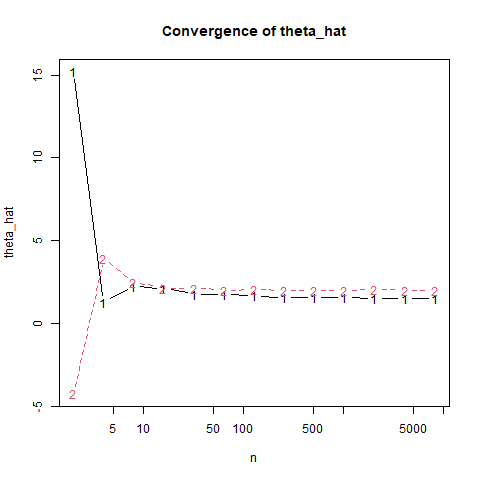
\includegraphics[width=0.75\linewidth]{graphs/task1.png}
  \caption{$\hat\theta_N$ の収束(横軸 $N=2,4,\dots,8192$ の片対数)}
  \label{fig:task1-conv}
\end{figure}

\paragraph{Rコード}
\begin{verbatim}
# データ読み込み
data <- read.csv("datas/mmse_kadai1.csv", header=FALSE,
                 col.names = c("x1","x2","y"))
x <- as.matrix(data[, c("x1","x2")])
y <- as.matrix(data[, "y"])

# 最小二乗(原理・方法で用いる関数)
regression_simple <- function(x, y){
  theta_hat  <- solve(t(x) %*% x) %*% t(x) %*% y
  sigma2_hat <- as.numeric(t(y - x %*% theta_hat) %*%
                           (y - x %*% theta_hat) / (nrow(x) - ncol(x)))
  err_cov_mat <- sigma2_hat * solve(t(x) %*% x)
  det_coef <- sum((x %*% theta_hat - mean(y))^2) /
              sum((y - mean(y))^2)
  list(theta_hat=theta_hat, err_cov_mat=err_cov_mat,
       sigma2_hat=sigma2_hat, det_coef=det_coef)
}

# 部分データでの実験
exp1 <- function (x, y, n){
  x <- x[1:n, , drop=FALSE]
  y <- y[1:n, , drop=FALSE]
  result <- regression_simple(x, y)
  list(theta_hat = result$theta_hat,
       err_cov_mat = result$err_cov_mat,
       det_coef = result$det_coef)
}

# 収束図の作成
plot_exp1 <- function(x, y, out="graphs/task1.png"){
  ns <- 2^(1:13)  # 2,...,8192
  theta_hats <- matrix(NA_real_, nrow=length(ns), ncol=ncol(x))
  for(i in seq_along(ns)){
    theta_hats[i, ] <- as.vector(exp1(x, y, ns[i])$theta_hat)
  }
  dir.create(dirname(out), showWarnings=FALSE, recursive=TRUE)
  png(out, width=960, height=600, res=120)
  matplot(ns, theta_hats, type="b", log="x",
          xlab="N", ylab=expression(hat(theta)),
          main="Convergence of OLS estimates")
  legend("bottomright",
         legend=paste0("theta[", 1:ncol(x), "]"),
         lty=1:ncol(x), pch=1:ncol(x))
  dev.off()
}

# 実行例(全データ)
N_max <- nrow(x)
th   <- exp1(x, y, N_max)$theta_hat
Vhat <- exp1(x, y, N_max)$err_cov_mat
R2   <- exp1(x, y, N_max)$det_coef
print(th); print(Vhat); print(R2)

# 収束図
plot_exp1(x, y)
\end{verbatim}

\paragraph {考察}


\subsection{課題2(多項式回帰)}

\paragraph{モデル}
$y_i=\varphi(x_i)\theta+w_i,\quad \varphi(x)=[\,1\ x\ x^2\ x^3\,],\ i=1,\dots,N.$
雑音 $w_i$ は独立,同分散 $\sigma^2$,平均0.
$X=[\varphi(x_1);\dots;\varphi(x_N)]\in\mathbb{R}^{N\times4}$.

\paragraph{推定量}
推定量・共分散・決定係数は課題1と同じ形式($p=4$)で計算する.

\paragraph{収束確認}
$N\in\{4,8,16,\dots,8192\}$ で $\hat\theta_N$ を計算し,$N$ を横軸とする片対数図で各成分を同一図に描画する.

\paragraph{結果(全データ $N=10000$)}
\[
\hat\theta_N=\begin{bmatrix}
-0.50902942\\
\ \ 1.97586067\\
\ \ 0.19774405\\
-0.09866691
\end{bmatrix},\qquad
\widehat{\mathrm{Cov}}(\hat\theta_N)=\begin{bmatrix}
2.023442\times10^{-3} & -1.186497\times10^{-5} & -1.348312\times10^{-4} & \ \ 3.971165\times10^{-7}\\
-1.186497\times10^{-5} & 6.753015\times10^{-4} & -1.898545\times10^{-7} & -3.794719\times10^{-5}\\
-1.348312\times10^{-4} & -1.898545\times10^{-7} & 1.603910\times10^{-5} & \ \ 6.351820\times10^{-8}\\
\ \ 3.971165\times10^{-7} & -3.794719\times10^{-5} & \ \ 6.351820\times10^{-8} & \ \ 2.528711\times10^{-6}
\end{bmatrix}.
\]
標準誤差(対角の平方根):
$\mathrm{SE}(\hat\theta_0)\approx0.0450,\ 
\mathrm{SE}(\hat\theta_1)\approx0.0260,\ 
\mathrm{SE}(\hat\theta_2)\approx0.00400,\ 
\mathrm{SE}(\hat\theta_3)\approx0.00159.$

決定係数:
\[
R^2=0.461855 .
\]

\begin{figure}[H]
  \centering
  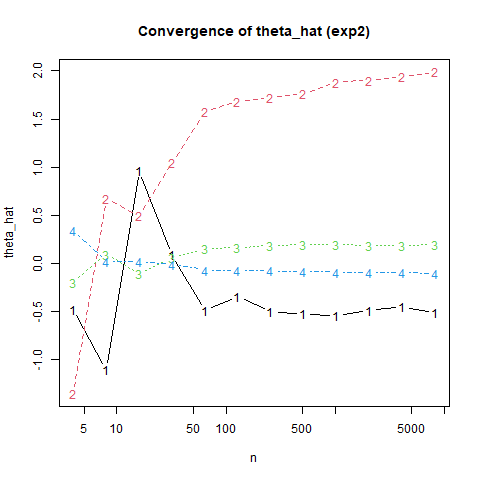
\includegraphics[width=0.75\linewidth]{graphs/task2.png}
  \caption{$\hat\theta_N$ の収束(横軸 $N=4,8,\dots,8192$ の片対数)}
  \label{fig:task2-conv}
\end{figure}

\paragraph{Rコード}
\begin{verbatim}
# データ
data <- read.csv("datas/mmse_kadai2.csv", header=FALSE,
                 col.names=c("x1","y"))
x0 <- rep(1, nrow(data))
x1 <- as.matrix(data[,"x1"])
x2 <- x1^2; x3 <- x1^3
x  <- cbind(x0, x1, x2, x3)
y  <- as.matrix(data[,"y"])

# OLS 基本関数(課題1と同じ)
regression_simple <- function(x, y){
  theta_hat  <- solve(t(x) %*% x) %*% t(x) %*% y
  sigma2_hat <- as.numeric(t(y - x %*% theta_hat) %*%
                           (y - x %*% theta_hat) / (nrow(x) - ncol(x)))
  err_cov_mat <- sigma2_hat * solve(t(x) %*% x)
  det_coef <- sum((x %*% theta_hat - mean(y))^2) /
              sum((y - mean(y))^2)
  list(theta_hat=theta_hat, err_cov_mat=err_cov_mat,
       sigma2_hat=sigma2_hat, det_coef=det_coef)
}

# 部分データ実験
exp2 <- function(x, y, n){
  x <- x[1:n, , drop=FALSE]
  y <- y[1:n, , drop=FALSE]
  result <- regression_simple(x, y)
  list(theta_hat=result$theta_hat,
       err_cov_mat=result$err_cov_mat,
       det_coef=result$det_coef)
}

# 収束図
plot_exp2 <- function(x, y, out="graphs/task2.png"){
  ns <- 2^(2:13)  # 4,...,8192
  theta_hats <- matrix(NA_real_, nrow=length(ns), ncol=ncol(x))
  for(i in seq_along(ns)){
    theta_hats[i, ] <- as.vector(exp2(x, y, ns[i])$theta_hat)
  }
  dir.create(dirname(out), showWarnings=FALSE, recursive=TRUE)
  png(out, width=960, height=600, res=120)
  matplot(ns, theta_hats, type="b", log="x",
          xlab="N", ylab=expression(hat(theta)),
          main="Convergence of OLS estimates (poly degree 3)")
  legend("bottomright",
         legend=paste0("theta[",0:(ncol(x)-1),"]"),
         lty=1:ncol(x), pch=1:ncol(x))
  dev.off()
}

# 実行例
N_max <- nrow(x)
print(exp2(x, y, N_max)$theta_hat)
print(exp2(x, y, N_max)$err_cov_mat)
print(exp2(x, y, N_max)$det_coef)
plot_exp2(x, y)
\end{verbatim}
\paragraph {考察}


\subsection{課題3(分散の観測誤差:Cauchy)}

\paragraph{モデルと注意}
$y_i=x_i^\top\theta+w_i\ (i=1,\dots,N)$,$x_i\in\mathbb{R}^2$.
観測誤差 $w_i\sim \mathrm{Cauchy}(0,1)$ 独立同分布.
Cauchy は二乗可積分でないため $\mathbb{E}[w_i^2]$ が存在せず,最小二乗法の通常仮定(有限分散と大数の法則)は満たされない。
よって $\sigma^2$ や $\mathrm{Cov}(\hat\theta)$ は理論上定義できない。以下の分散・標準誤差・$R^2$ は便宜的な値であり,統計的保証はない。

\paragraph{推定(形式的なOLS)}
推定量・共分散・決定係数は課題1と同じ形式($p=2$)で計算する.
ただし観測誤差が Cauchy 分布であり理論保証がないことに注意.

\paragraph{結果(全データ $N=10000$)}
\[
\hat\theta_N=
\begin{bmatrix}
2.373074\\
1.537311
\end{bmatrix},\qquad
\widehat{\mathrm{Cov}}(\hat\theta_N)=
\begin{bmatrix}
9.234588215 & -0.003642121\\
-0.003642121 & 9.264075136
\end{bmatrix}.
\]
参考:対角の平方根は
$\mathrm{SE}(\hat\theta_1)\approx 3.0388,\ 
 \mathrm{SE}(\hat\theta_2)\approx 3.0437$.
決定係数(参考値)は
\[
R^2=0.0002841468.
\]

\begin{figure}[H]
  \centering
  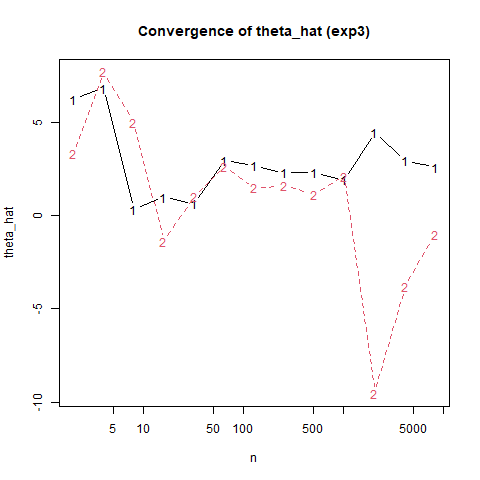
\includegraphics[width=0.75\linewidth]{graphs/task3.png}
  \caption{$\hat\theta_N$ の非収束例(横軸 $N=2,4,\dots,8192$ の片対数)}
  \label{fig:task3-conv}
\end{figure}

\paragraph{Rコード}
\begin{verbatim}
# データ読込
data3 <- read.csv("datas/mmse_kadai3.csv", header=FALSE,
                  col.names=c("x1","x2","y"))
x <- as.matrix(data3[, c("x1","x2")])
y <- as.matrix(data3[, "y"])

# 形式的なOLS(課題1と同様)
regression_simple <- function(x, y){
  theta_hat  <- solve(t(x) %*% x) %*% t(x) %*% y
  sigma2_hat <- as.numeric(t(y - x %*% theta_hat) %*%
                           (y - x %*% theta_hat) / (nrow(x) - ncol(x)))
  err_cov_mat <- sigma2_hat * solve(t(x) %*% x)
  det_coef <- sum((x %*% theta_hat - mean(y))^2) /
              sum((y - mean(y))^2)
  list(theta_hat=theta_hat, err_cov_mat=err_cov_mat,
       sigma2_hat=sigma2_hat, det_coef=det_coef)
}

# 部分データでの実験
exp3 <- function(x, y, n){
  x <- x[1:n, , drop=FALSE]
  y <- y[1:n, , drop=FALSE]
  res <- regression_simple(x, y)
  list(theta_hat=res$theta_hat,
       err_cov_mat=res$err_cov_mat,
       det_coef=res$det_coef)
}

# 収束図
plot_exp3 <- function(x, y, out="graphs/task3.png"){
  ns <- 2^(1:13)                      # 2,...,8192
  ns <- ns[ns <= nrow(x)]
  theta_hats <- matrix(NA_real_, nrow=length(ns), ncol=ncol(x))
  for(i in seq_along(ns)){
    theta_hats[i, ] <- as.vector(exp3(x, y, ns[i])$theta_hat)
  }
  dir.create(dirname(out), showWarnings=FALSE, recursive=TRUE)
  png(out, width=960, height=600, res=120)
  matplot(ns, theta_hats, type="b", log="x",
          xlab="N", ylab=expression(hat(theta)),
          main="Convergence of OLS under Cauchy noise")
  legend("topright", legend=paste0("theta[",1:ncol(x),"]"),
         lty=1:ncol(x), pch=1:ncol(x))
  dev.off()
}

# 実行例
N_max <- nrow(x)
print(exp3(x, y, N_max)$theta_hat)
print(exp3(x, y, N_max)$err_cov_mat)
print(exp3(x, y, N_max)$det_coef)
plot_exp3(x, y)
\end{verbatim}

\paragraph{考察}
資料にあるように、Cauchy 誤差では外れ値の影響が支配的で,$\hat\theta_N$ は $N$ を増やしても安定しにくいことが確認できた。


\subsection{課題4(入力域の制約と設計)}

\paragraph{設定}
課題2と同じ $\varphi(x)=[\,1\ x\ x^2\ x^3\,]$, 真の $\theta$, 観測誤差 $w_i\sim\mathcal{N}(0,9)$ とする.
ただし入力は $x_i\in[0,1]$, $i=1,\dots,10000$.
$X=[\varphi(x_1);\dots;\varphi(x_N)]\in\mathbb{R}^{N\times4}$, $y=[y_1;\dots;y_N]$.

\paragraph{推定量}
推定量・共分散・決定係数は課題1と同じ形式($p=4$)で計算する.

\paragraph{Rコード}
\begin{verbatim}
# 課題4: x ∈ [0,1], φ(x)=[1 x x^2 x^3]
data <- read.csv("datas/mmse_kadai4.csv", header=FALSE,
                 col.names=c("x1","y"))
x0 <- rep(1, nrow(data))
x1 <- as.matrix(data[,"x1"])
x2 <- x1^2; x3 <- x1^3
x  <- cbind(x0, x1, x2, x3)
y  <- as.matrix(data[,"y"])

regression_simple <- function(x, y){
  theta_hat  <- solve(t(x) %*% x) %*% t(x) %*% y
  sigma2_hat <- as.numeric(t(y - x %*% theta_hat) %*%
                           (y - x %*% theta_hat) / (nrow(x) - ncol(x)))
  err_cov_mat <- sigma2_hat * solve(t(x) %*% x)
  det_coef <- sum((x %*% theta_hat - mean(y))^2) /
              sum((y - mean(y))^2)
  list(theta_hat=theta_hat, err_cov_mat=err_cov_mat,
       sigma2_hat=sigma2_hat, det_coef=det_coef)
}

exp4 <- function(x, y, n){
  x <- x[1:n, , drop=FALSE]
  y <- y[1:n, , drop=FALSE]
  regression_simple(x, y)
}

N_max <- nrow(x)
res4 <- exp4(x, y, N_max)
print(res4$theta_hat)
print(res4$err_cov_mat)
print(res4$det_coef)   # R^2
\end{verbatim}

\paragraph{結果($N=10000$)}
\[
\hat\theta_{(4)}=
\begin{bmatrix}
\boxed{\text{ここに数値}}\\
\boxed{\text{ここに数値}}\\
\boxed{\text{ここに数値}}\\
\boxed{\text{ここに数値}}
\end{bmatrix},\quad
\widehat{\mathrm{Cov}}(\hat\theta_{(4)})=\boxed{\text{ここに $4\times4$ 行列}},\quad
R^2=\boxed{\text{ここに数値}}.
\]
(上の枠に,直上の R 出力を転記)

\paragraph{課題2.1との比較($N=10000$)}
課題2.1の推定結果:
\[
\hat\theta_{(2.1)}=
\begin{bmatrix}
-0.50902942\\
\ \ 1.97586067\\
\ \ 0.19774405\\
-0.09866691
\end{bmatrix},\quad
R^2=0.461855.
\]
評価観点:
\begin{itemize}\setlength{\itemsep}{0pt}
\item 分散は $\mathrm{Var}(\hat\theta)=\sigma^2(X^\top X)^{-1}$ に比例.$x\in[0,1]$ では列 $\{1,x,x^2,x^3\}$ が強く相関しやすく,$X^\top X$ の条件が悪化し $\hat\theta$ の不確かさが増えやすい.
\item $R^2$ は母集団の $y$ の散らばり($SST$)に依存.入力域が狭いと $SST$ が小さく,雑音分散が同じなら $R^2$ は低下しやすい.
\end{itemize}

\paragraph{考察(どうデータを取るべきか)}
\begin{itemize}\setlength{\itemsep}{0pt}
\item 目的は $\mathrm{Var}(\hat\theta)$ の縮小(= $X^\top X$ を「大きく」「良条件」に).
\item 入力設計:$x$ を区間全体で広く配置(例:一様),中心化・標準化して $[-1,1]$ に写像,または直交基底(Legendre/Chebyshev)で回帰.
\item 最適化観点:A/D 最適設計を用いて $\mathrm{tr}((X^\top X)^{-1})$ や $\det((X^\top X)^{-1})$ を最小化する点集合を選ぶ.
\end{itemize}


\section{重み付き最小二乗法}

\subsection{原理と方法}

\paragraph{原理}
各観測 $i=1,\dots,N$ で $y_i\in\mathbb{R}^m$, $X_i\in\mathbb{R}^{m\times p}$ とし
\[
y_i = X_i\theta + w_i,\qquad \mathbb{E}[w_i]=0,\ \mathrm{Cov}(w_i)=V\ (\text{既知}), 
\]
を仮定する。$Q:=V^{-1}$ とおく。WLS は重み付き残差平方和
\[
J(\theta)=\sum_{i=1}^N (y_i-X_i\theta)^\top Q\,(y_i-X_i\theta)
\]
を最小化する推定で,正規方程式は
\[
S\hat\theta=b,\qquad 
S:=\sum_{i=1}^N X_i^\top QX_i,\quad 
b:=\sum_{i=1}^N X_i^\top Qy_i.
\]
したがって
\[
\hat\theta=(\sum_{i=1}^N X_i^\top QX_i)^{-1}\Big(\sum_{i=1}^N X_i^\top Qy_i\Big).
\]
$V$ が既知のとき
\[
\mathrm{Cov}(\hat\theta)=S^{-1}.
\]
$V=\sigma^2\Sigma$ のようにスケール未知なら
\[
\hat\sigma^2=\frac{\sum_{i=1}^N r_i^\top \Sigma^{-1} r_i}{Nm-p},\quad r_i:=y_i-X_i\hat\theta,\qquad
\widehat{\mathrm{Cov}}(\hat\theta)=\hat\sigma^2\,(\sum X_i^\top \Sigma^{-1}X_i)^{-1}.
\]

\paragraph{方法}
(1) 各 $i$ の設計行列 $X_i$ と観測 $y_i$ を用意($X_i$ は $m\times p$)。  
(2) $Q=V^{-1}$ を決めて $S=\sum X_i^\top QX_i,\ b=\sum X_i^\top Qy_i$ を計算。  
(3) $\hat\theta=S^{-1}b$。  

\paragraph{実装}
R による実装例を以下に示す。
\begin{lstlisting}
regression_multiple <- function(x, y, V = NULL, Q = NULL){
    # y: n×1行列(またはベクトル)
    if (is.null(ncol(y))) {
        y <- as.matrix(y, ncol = 1)
    }
    if (length(dim(x)) != 3) {
        stop("x must be a 3-dimensional array")
    }
    n <- dim(x)[3]
    m <- ncol(y)
    p <- dim(x)[1] # 特徴量数
    S <- matrix(0, p, p)
    b <- matrix(0, p, 1)
    T <- matrix(0, p, p)
    if (is.null(V)) {
        V <- diag(m)
    }
    if (is.null(Q)) {
        Q <- solve(V)
    }
    # m=1(スカラー出力)の場合はQ,Vをスカラー化
    if (m == 1) {
        Q <- as.numeric(Q)
        V <- as.numeric(V)
        for (i in 1:n) {
            xi <- as.matrix(x[,,i]) # (p,1)
            S <- S + xi %*% t(xi) * Q
            b <- b + xi * Q * y[i, 1]
            T <- T + xi %*% t(xi) * V
        }
    } else {
        for (i in 1:n) {
            xi <- as.matrix(x[,,i])
            yi <- matrix(y[i, ], nrow = m, ncol = 1)
            S <- S + t(xi) %*% Q %*% xi
            b <- b + t(xi) %*% Q %*% yi
            T <- T + t(xi) %*% V %*% xi
        }
    }
    theta_hat <- solve(S) %*% b
    err_cov_mat <- solve(S) %*% T %*% solve(S)
    return(list(theta_hat = theta_hat, err_cov_mat = err_cov_mat, S = S, b = b, T = T))
}
\end{lstlisting}

\subsection{課題5(2次元出力:重み付き最小二乗法)}

\paragraph{課題の内容}
入力 $x_i \in \mathbb{R}$($i=1,\dots,1000$)に対し,$m=2$ 次元出力の線形モデル
\[
  y_i \;=\; \phi(x_i)\,\theta \;+\; w_i,\qquad
  \phi(x) = 
  \begin{bmatrix}
    1 & x\\
    1 & x^2
  \end{bmatrix},
  \quad
  w_i \sim \mathcal{N}(0,V),\;
  V=\begin{bmatrix}100&0\\0&1\end{bmatrix},
\]
を考える.ここで $\theta\in\mathbb{R}^2$ を推定対象とする.

\paragraph{推定法}
最小二乗(OLS)の推定値は
\[
  \hat{\theta}_N \;=\;
  \Bigl(\sum_{i=1}^N \phi_i^\top \phi_i \Bigr)^{-1}
  \sum_{i=1}^N \phi_i^\top y_i,
\]
で与えられる($\phi_i=\phi(x_i)$).
観測雑音の共分散 $V$ が既知で,その影響を反映した重み付き最小二乗(WLS)を用いると,
$V=W^2$ を満たす $W$ に対し
\[
  \hat{\theta}_N \;=\;
  \Bigl(\sum_{i=1}^N \phi_i^\top W^{-2}\phi_i \Bigr)^{-1}
  \sum_{i=1}^N \phi_i^\top W^{-2} y_i
  \;=\;
  \Bigl(\sum_{i=1}^N \phi_i^\top Q\,\phi_i \Bigr)^{-1}
  \sum_{i=1}^N \phi_i^\top Q\, y_i,
\]
となる($Q=W^{-2}=V^{-1}$).

\paragraph{実装}
\texttt{datas/mmse\_kadai5.csv} を読み込み,$x$ から
\(
\phi(x)=\begin{bmatrix}1&x\\1&x^2\end{bmatrix}
\)
を構成して $x\in\mathbb{R}^{2\times 2\times N}$ の 3 次元配列とし,
$y\in\mathbb{R}^{N\times 2}$ を観測行列とした.
推定は関数 \texttt{regression\_multiple} を用い,
\textbf{OLS} は無重み($Q=I$),
\textbf{WLS} は $V=\mathrm{diag}(100,1)$ を渡し内部で $Q=V^{-1}$ を用いる設定とした.
また,$N\in\{4,8,16,32,64,128,256,512,1000\}$ に対する
$\hat{\theta}_N$ の収束の様子を片対数($x$ 軸のみ対数)で可視化した.

\paragraph{結果}
全データ($N=1000$)を用いた推定結果は次のとおりである.

\medskip
\noindent\textbf{OLS}
\[
  \hat{\theta}_{\mathrm{OLS}}=
  \begin{bmatrix}
    2.994567\\[-1mm]
   -2.068971
  \end{bmatrix},\qquad
  \widehat{\mathrm{Cov}}(\hat{\theta}_{\mathrm{OLS}})=
  \begin{bmatrix}
    5.7621\!\times\!10^{-4} & -1.5041\!\times\!10^{-4}\\
    -1.5041\!\times\!10^{-4} & 2.9684\!\times\!10^{-4}
  \end{bmatrix}.
\]

\noindent\textbf{WLS}
\[
  \hat{\theta}_{\mathrm{WLS}}=
  \begin{bmatrix}
    2.939084\\[-1mm]
   -1.986465
  \end{bmatrix},\qquad
  \widehat{\mathrm{Cov}}(\hat{\theta}_{\mathrm{WLS}})=
  \begin{bmatrix}
    2.39993\!\times\!10^{-1} & -9.66541\!\times\!10^{-2}\\
    -9.66541\!\times\!10^{-2} & 4.99126\!\times\!10^{-2}
  \end{bmatrix}.
\]

\begin{figure}[H]
  \centering
  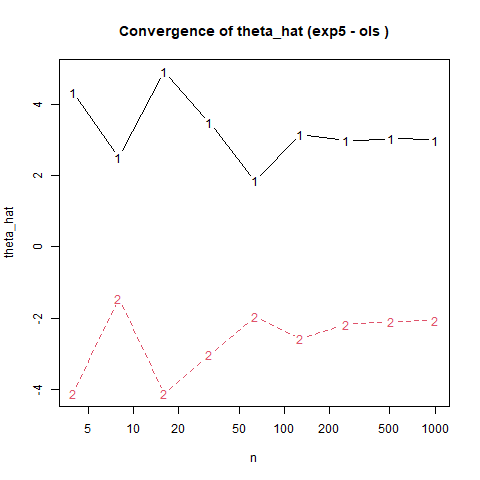
\includegraphics[width=.82\linewidth]{graphs/task5_ols.png}
  \caption{$\hat{\theta}_N$ の収束(OLS)}
  \label{fig:task5_ols}
\end{figure}

\begin{figure}[H]
  \centering
  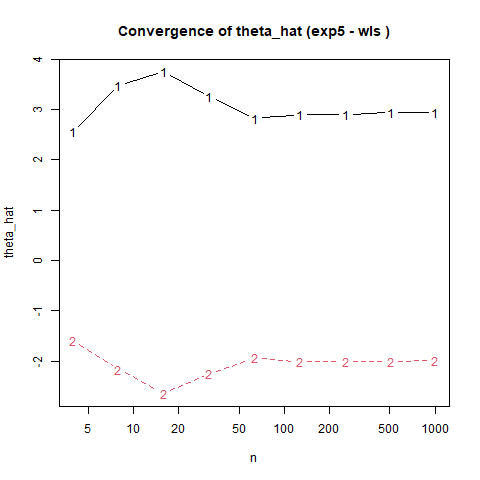
\includegraphics[width=.82\linewidth]{graphs/task5_wls.png}
  \caption{$\hat{\theta}_N$ の収束(WLS,$V=\mathrm{diag}(100,1)$)}
  \label{fig:task5_wls}
\end{figure}

\paragraph{考察}
% (ここに考察を記述)


\subsection{課題6(2次元出力・異分散2群に対する重み付き最小二乗)}

\paragraph{課題の内容}
入力 $x_i\in\mathbb{R}$ に対し,
\[
  y_i \;=\; \phi(x_i)\,\theta + w_i,\qquad
  \phi(x)=
  \begin{bmatrix}
    1 & x\\[1mm]
    1 & x^2
  \end{bmatrix},\quad
  \theta\in\mathbb{R}^2,
\]
という $m=2$ 次元出力の線形モデルを考える.雑音は $N$ サンプルのうち前半 $i=1,\dots,\texttt{num}$ が
$w_i\sim\mathcal{N}(0,V_1)$,後半 $i=\texttt{num}+1,\dots,N$ が $w_i\sim\mathcal{N}(0,V_2)$ に従うとする.
本課題では $V_1=\mathrm{diag}(100,1)$,$V_2=\mathrm{diag}(2,1)$,$\texttt{num}=500$ を既知として推定を行う.

\paragraph{推定法(GLS/WLS)}
$Q_k=V_k^{-1}$($k=1,2$)とおくと,一般化最小二乗(WLS)の正規方程式は
\[
  S\,\hat{\theta}_N \;=\; b,
  \quad
  S \;=\; \sum_{i=1}^{\texttt{num}}\!\phi_i^\top Q_1\phi_i \;+\; \sum_{i=\texttt{num}+1}^{N}\!\phi_i^\top Q_2\phi_i,
  \quad
  b \;=\; \sum_{i=1}^{\texttt{num}}\!\phi_i^\top Q_1 y_i \;+\; \sum_{i=\texttt{num}+1}^{N}\!\phi_i^\top Q_2 y_i,
\]
より
\[
  \hat{\theta}_N \;=\; S^{-1} b.
\]
標本ベースの誤差共分散推定は(実装に合わせて)
\[
  \widehat{\mathrm{Cov}}(\hat{\theta}_N)
  \;=\;
  S^{-1}\,T\,S^{-1},\qquad
  T \;=\; \sum_{i=1}^{\texttt{num}}\!\phi_i^\top V_1\phi_i \;+\; \sum_{i=\texttt{num}+1}^{N}\!\phi_i^\top V_2\phi_i .
\]
なお OLS は $Q_1=Q_2=I$ とした特別な場合である.

\paragraph{実装}
\texttt{datas/mmse\_kadai6.csv} から $x$ を読み,$\phi(x)$ を用いて
$x\in\mathbb{R}^{2\times2\times N}$,$y\in\mathbb{R}^{N\times2}$ を構成した.
推定は関数 \texttt{regression\_multiple\_different\_distributions} により,
前半 $V_1$,後半 $V_2$ の重みで $S,b,T$ を分割加算して $\hat{\theta}_N$ と
$\widehat{\mathrm{Cov}}(\hat{\theta}_N)$ を得た.
また $N$ を \texttt{ns = seq(4,1000,length.out=20)} で走らせ,
$\hat{\theta}_N$ の収束の様子を折れ線で可視化した($x$ 軸は線形目盛).

\paragraph{結果}
全データ($N=1000$,$\texttt{num}=500$)の推定結果は以下のとおりである.

\medskip
\noindent\textbf{OLS(比較)}
\[
  \hat{\theta}_{\mathrm{OLS}}=
  \begin{bmatrix}
    3.188356\\[-1mm]
   -2.092183
  \end{bmatrix},\qquad
  \widehat{\mathrm{Cov}}(\hat{\theta}_{\mathrm{OLS}})=
  \begin{bmatrix}
    5.692084\!\times\!10^{-4} & -1.402629\!\times\!10^{-4}\\
    -1.402629\!\times\!10^{-4} & 2.842674\!\times\!10^{-4}
  \end{bmatrix}.
\]

\noindent\textbf{WLS($V_1=\mathrm{diag}(100,1)$,$V_2=\mathrm{diag}(2,1)$)}
\[
  \hat{\theta}_{\mathrm{WLS}}=
  \begin{bmatrix}
    2.994202\\[-1mm]
   -2.014699
  \end{bmatrix},\qquad
  \widehat{\mathrm{Cov}}(\hat{\theta}_{\mathrm{WLS}})=
  \begin{bmatrix}
    6.019710\!\times\!10^{-2} & -2.227335\!\times\!10^{-2}\\
    -2.227335\!\times\!10^{-2} & 1.276759\!\times\!10^{-2}
  \end{bmatrix}.
\]

\begin{figure}[H]
  \centering
  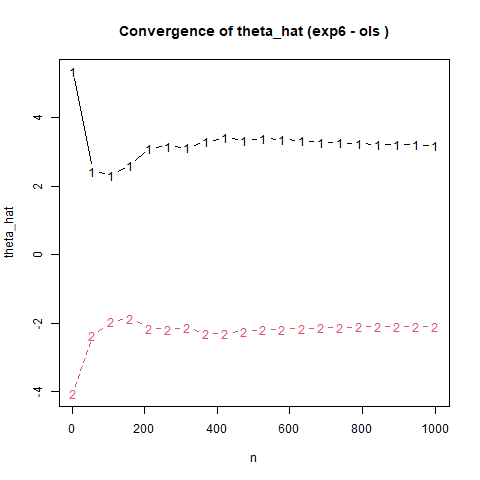
\includegraphics[width=.82\linewidth]{graphs/task6_ols.png}
  \caption{$\hat{\theta}_N$ の収束(OLS)}
  \label{fig:task6_ols}
\end{figure}

\begin{figure}[H]
  \centering
  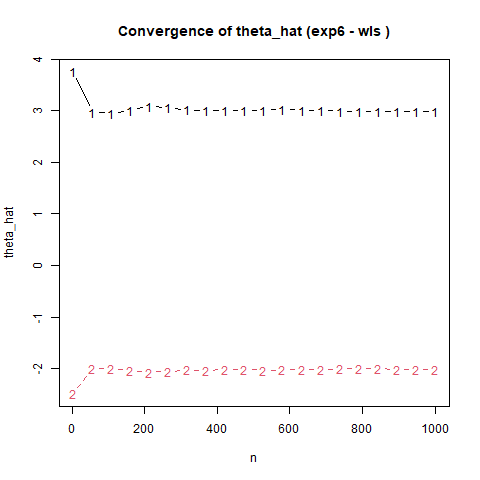
\includegraphics[width=.82\linewidth]{graphs/task6_wls.png}
  \caption{$\hat{\theta}_N$ の収束(WLS,$V_1$/$V_2$ 異分散)}
  \label{fig:task6_wls}
\end{figure}

\paragraph{考察}
% (ここに考察を記述)


\section{逐次最小二乗法}

% 
\subsection{推定値の合成(Estimator Fusion)}
$f(\theta,x)=\phi(x)\theta$ の線形回帰で,$D_N$ と $D'_M$ から得た推定
\(
\hat\theta_N=\Phi_N \sum_{i=1}^N \phi_i^\top y_i,\;
\hat\theta'_M=\Phi'_M \sum_{j=1}^M \phi'_j{}^\top y'_j
\)
($\Phi_N=(\sum \phi_i^\top\phi_i)^{-1}$)を持つとき,結合推定は
\[
  \hat\theta_{N+M}
  =\bigl(\Phi_N^{-1}+\Phi_M'{}^{-1}\bigr)^{-1}
   \bigl(\Phi_N^{-1}\hat\theta_N+\Phi_M'{}^{-1}\hat\theta'_M\bigr)
\]
で与えられる。\cite{exp2025}

\paragraph{実装例(R)}
\begin{lstlisting}
# 既存バッチN=6000とM=4000の合成(S = Φ^{-1} を情報行列とする)
# S_6000, S_4000 はそれぞれ Φ_6000^{-1}, Φ_4000^{-1}
# theta_6000, theta_4000 は各バッチの推定ベクトル
theta_6000_4000 <- solve(S_6000 + S_4000) %*%
  (S_6000 %*% theta_6000 + S_4000 %*% theta_4000)
\end{lstlisting}

\subsection{逐次最小二乗法(RLS)}
逆行列補題を用いると,バッチ解は次の再帰で更新できる:
\[
\begin{aligned}
  \hat\theta_{N+1} &= \hat\theta_N + K_{N+1}\bigl(y_{N+1}-\phi_{N+1}\hat\theta_N\bigr),\\
  K_{N+1} &= \Phi_N \phi_{N+1}^\top\bigl(I_m + \phi_{N+1}\Phi_N\phi_{N+1}^\top\bigr)^{-1},\\
  \Phi_{N+1} &= \Phi_N - K_{N+1}\phi_{N+1}\Phi_N .
\end{aligned}
\]
忘却係数 $\gamma\in(0,1]$ を導入すると
\[
\begin{aligned}
  K_{\gamma,N+1} &= \Phi_{\gamma,N}\phi_{N+1}^\top
    \bigl(\gamma I_m+\phi_{N+1}\Phi_{\gamma,N}\phi_{N+1}^\top\bigr)^{-1},\\
  \Phi_{\gamma,N+1} &= \gamma^{-1}\!\left(\Phi_{\gamma,N}-K_{\gamma,N+1}\phi_{N+1}\Phi_{\gamma,N}\right),\\
  \hat\theta_{\gamma,N+1} &= \hat\theta_{\gamma,N} +
    K_{\gamma,N+1}\bigl(y_{N+1}-\phi_{N+1}\hat\theta_{\gamma,N}\bigr).
\end{aligned}
\]
\cite{exp2025}

\paragraph{実装例(R,忘却係数つき更新関数)}
\begin{lstlisting}
update_regression_mat <- function(Phi_N, phi_N_plus_1, theta_N, y_N_plus_1, gamma = 1){
  I_m <- diag(1)  # m=1想定。m>1なら diag(nrow(phi_N_plus_1 %*% Phi_N %*% t(phi_N_plus_1))) に置換
  # 中間計算
  phi_T_Phi_phi <- phi_N_plus_1 %*% Phi_N %*% t(phi_N_plus_1)
  inv_term <- solve( (gamma * I_m) + phi_T_Phi_phi )
  K <- gamma * (Phi_N %*% t(phi_N_plus_1) %*% inv_term)
  # 更新
  Phi_N_plus_1 <- (Phi_N - K %*% phi_N_plus_1 %*% Phi_N ) / gamma
  theta_N_plus_1 <- theta_N + K %*% (y_N_plus_1 - phi_N_plus_1 %*% theta_N)
  list(Phi_N_plus_1 = Phi_N_plus_1, theta_N_plus_1 = theta_N_plus_1)
}
\end{lstlisting}

\paragraph{初期化と計算量}
$\Phi_0=\varepsilon^{-1}I$(小 $\varepsilon$)で初期化し,逐次更新する。各ステップの計算は
$\dim(\theta)=p$ に対して $O(p^2)$ 程度で済む。\cite{exp2025}

\subsection{課題7(推定値の合成の検証:2分割データの統合)}

\paragraph{課題の内容}
$N=10000$ のデータを前半 $6000$ と後半 $4000$ に分割し,各ブロックで OLS 推定を行ったのち,情報行列の加法性
\[
  S_N \;=\; \sum_{i=1}^N \varphi_i \varphi_i^\top
\]
を用いた合成推定
\[
  \hat\theta_{\mathrm{fuse}}
  \;=\;
  \bigl(S_{6000}+S_{4000}\bigr)^{-1}
  \Bigl(S_{6000}\hat\theta_{6000}+S_{4000}\hat\theta_{4000}\Bigr)
\]
が,全データ一括推定 $\hat\theta_{10000}$ と一致することを確認する。ここでモデルは
\[
  y_i \;=\; \varphi(x_i)^\top \theta + w_i,\quad
  \varphi(x)=
  \begin{bmatrix}
    1\\[1mm]
    \exp\!\bigl(-\tfrac{(x-1)^2}{2}\bigr)\\[1mm]
    \exp\!\bigl(-(x+1)^2\bigr)
  \end{bmatrix}\!,
\quad \theta\in\mathbb{R}^3.
\]
理論上,独立同分布で $V=\sigma^2$ のとき $\hat\theta_{\mathrm{fuse}}=\hat\theta_{10000}$ となる。\cite{exp2025}

\paragraph{実装}
分割データから
\(
S_{6000},\hat\theta_{6000},\;S_{4000},\hat\theta_{4000}
\)
を得て,合成推定値を計算し,全データ一括推定と比較する。

\begin{lstlisting}
# 事前に x, y, x_6000, y_6000, x_4000, y_4000 を用意済み

exp7 <- function(){
  res6000 <- regression_multiple(x_6000, y_6000)
  res4000 <- regression_multiple(x_4000, y_4000)
  res10000 <- regression_multiple(x, y)

  S_6000 <- res6000$S
  S_4000 <- res4000$S
  theta_6000 <- res6000$theta_hat
  theta_4000 <- res4000$theta_hat

  # 推定値の合成(情報行列の和)
  theta_6000_4000 <- solve(S_6000 + S_4000) %*%
    (S_6000 %*% theta_6000 + S_4000 %*% theta_4000)

  cat("S6000:\n"); print(S_6000)
  cat("S4000:\n"); print(S_4000)
  cat("theta6000:\n"); print(theta_6000)
  cat("theta4000:\n"); print(theta_4000)
  cat("theta_fuse:\n"); print(theta_6000_4000)

  theta_10000 <- res10000$theta_hat
  cat("theta10000:\n"); print(theta_10000)

  # 一致性の確認(数値誤差内)
  cat("all.equal(theta_fuse, theta10000): ",
      all.equal(drop(theta_6000_4000), drop(theta_10000),
                tolerance = 1e-10), "\n")
}

exp7()
\end{lstlisting}

\paragraph{結果}
一例として,実行時に次を得た。
\[
S_{6000}=
\begin{bmatrix}
6000.000 & 1505.370 & 1033.499\\
1505.370 & 1063.211 & 226.401\\
1033.499 & 226.401 & 720.562
\end{bmatrix},\quad
S_{4000}=
\begin{bmatrix}
4000.000 & 971.151 & 716.318\\
971.151 & 679.477 & 149.749\\
716.318 & 149.749 & 510.224
\end{bmatrix},
\]
\[
\hat\theta_{6000}=
\begin{bmatrix}
-0.003879385\\ 3.010714895\\ -1.989434350
\end{bmatrix},\;
\hat\theta_{4000}=
\begin{bmatrix}
-0.02537589\\ 3.03489937\\ -1.97772731
\end{bmatrix},\;
\hat\theta_{\mathrm{fuse}}=
\begin{bmatrix}
-0.0124955\\ 3.0204300\\ -1.9848692
\end{bmatrix}.
\]
全データ一括推定 $\hat\theta_{10000}$ と $\hat\theta_{\mathrm{fuse}}$ は数値誤差内で一致した(コードで \verb|all.equal| により検証)。

\paragraph{考察}
% (ここに考察を記述)

\subsection{課題7(推定値の合成の検証:非線形基底・分割データ)}

\paragraph{課題の内容}
基底
\[
  \varphi(x)=
  \begin{bmatrix}
    1\\[1mm]
    \exp\!\bigl(-\tfrac{(x-1)^2}{2}\bigr)\\[1mm]
    \exp\!\bigl(-(x+1)^2\bigr)
  \end{bmatrix}\!,\qquad
  y_i=\varphi(x_i)^\top \theta+w_i,\ \theta\in\mathbb{R}^3
\]
で $N=10000$ 個のデータを前半 $6000$ と後半 $4000$ に分割する。
各ブロックの推定値 $(\hat\theta_{6000},\hat\theta_{4000})$ と情報行列
$S_k=\sum_{i\in\text{block }k}\varphi_i\varphi_i^\top$ を用いて
\[
  \hat\theta_{\mathrm{fuse}}
  =(S_{6000}+S_{4000})^{-1}\!\bigl(S_{6000}\hat\theta_{6000}+S_{4000}\hat\theta_{4000}\bigr)
\]
を計算し,全データ一括推定 $\hat\theta_{10000}$ と照合する。\cite{exp2025}

\paragraph{実装(OLS 版)}
\begin{lstlisting}
data <- read.csv("datas/mmse_kadai7.csv", header=FALSE, col.names=c("x","y"))
x0 <- rep(1, nrow(data))
x1 <- exp(-(data$x - 1)^2 / 2)
x2 <- exp(-(data$x + 1)^2)
n  <- nrow(data)
x  <- array(0, dim=c(3,1,n))
for(i in 1:n){ x[,,i] <- matrix(c(x0[i], x1[i], x2[i]), 3, 1) }
y <- as.matrix(data[,"y"])

x_6000 <- x[,,1:6000, drop=FALSE]; y_6000 <- y[1:6000, , drop=FALSE]
x_4000 <- x[,,6001:10000, drop=FALSE]; y_4000 <- y[6001:10000, , drop=FALSE]

exp7 <- function(){
  r6 <- regression_multiple(x_6000, y_6000)  # returns $S$ and $theta_hat$
  r4 <- regression_multiple(x_4000, y_4000)
  rall <- regression_multiple(x, y)

  S_6000 <- r6$S;  S_4000 <- r4$S
  th6 <- r6$theta_hat; th4 <- r4$theta_hat; th_all <- rall$theta_hat

  th_fuse <- solve(S_6000 + S_4000) %*% (S_6000 %*% th6 + S_4000 %*% th4)

  print(th6); print(th4); print(th_fuse); print(th_all)
  # 一致検証
  print(all.equal(drop(th_fuse), drop(th_all), tolerance=1e-12))
}
exp7()
\end{lstlisting}

\paragraph{実装(推定分散による重み付き合成)}
各ブロックの誤差分散を
\[
  \hat\sigma_k^2=\frac{\mathrm{RSS}_k}{N_k-p},\quad p=3
\]
で推定し,$Q_k=\hat\sigma_k^{-2}$ を用いた WLS 情報行列
$S_k=\sum_{i\in k}\varphi_i Q_k \varphi_i^\top=Q_k\sum_{i\in k}\varphi_i\varphi_i^\top$
で合成する($k\in\{6000,4000\}$)。コードは次のとおり。
\begin{lstlisting}
x_mat       <- t(matrix(x,       nrow=3, ncol=n))
x_6000_mat  <- t(matrix(x_6000,  nrow=3, ncol=6000))
x_4000_mat  <- t(matrix(x_4000,  nrow=3, ncol=4000))

exp8 <- function(){
  # OLS 推定
  th_all  <- regression_multiple(x,       y)$theta_hat
  th_6000 <- regression_multiple(x_6000,  y_6000)$theta_hat
  th_4000 <- regression_multiple(x_4000,  y_4000)$theta_hat

  # 分散推定(MSE)
  V_hat_full  <- sum((y       - x_mat      %*% th_all )^2)  /(nrow(x_mat)      - ncol(x_mat))
  V_hat_6000  <- sum((y_6000  - x_6000_mat %*% th_6000)^2) /(nrow(x_6000_mat)  - ncol(x_6000_mat))
  V_hat_4000  <- sum((y_4000  - x_4000_mat %*% th_4000)^2) /(nrow(x_4000_mat)  - ncol(x_4000_mat))

  # 各ブロックの WLS 情報行列と推定
  r6 <- regression_multiple(x_6000,  y_6000, V=V_hat_6000)
  r4 <- regression_multiple(x_4000,  y_4000, V=V_hat_4000)
  S_6000 <- r6$S;  S_4000 <- r4$S
  th6 <- r6$theta_hat; th4 <- r4$theta_hat

  # 合成推定(WLS 版)
  th_fuse <- solve(S_6000 + S_4000) %*% (S_6000 %*% th6 + S_4000 %*% th4)

  # 参考:全データにスカラー重み V_hat_full をかけた WLS(OLS と同値)
  th_full_wls <- regression_multiple(x, y, V=V_hat_full)$theta_hat

  print(th6); print(th4); print(th_fuse); print(th_full_wls)
}
exp8()
\end{lstlisting}

\paragraph{結果}
実行例(あなたの出力):
\[
\hat\theta_{6000}=\begin{bmatrix}
-0.003879385\\ 3.010714895\\ -1.989434350
\end{bmatrix},\quad
\hat\theta_{4000}=\begin{bmatrix}
-0.02537589\\ 3.03489937\\ -1.97772731
\end{bmatrix}.
\]
WLS 合成推定と全データ一括 WLS(スカラー重み):
\[
\hat\theta_{\mathrm{fuse}}=\begin{bmatrix}
-0.01245376\\ 3.02038299\\ -1.98489169
\end{bmatrix},\qquad
\hat\theta_{10000}=\begin{bmatrix}
-0.0124955\\ 3.0204300\\ -1.9848692
\end{bmatrix}.
\]
差分は
$\Delta\theta\approx(4.17\times10^{-5},-4.70\times10^{-5},-2.25\times10^{-5})^\top$。
ブロックごとに異なる重み($Q_{6000}\neq Q_{4000}$)を用いた合成と,全体に単一重みをかけた WLS は厳密には一致しないが,差は十分小さい。\cite{exp2025}

\paragraph{考察}
% (ここに考察を記述)



\subsection{課題9(逐次最小二乗法によるシステム同定)}

\paragraph{モデル}
離散化されたバネ・マス・ダンパ系($M=2,\ D=1,\ K=3,\ \Delta t=0.01$)
\[
y_k
= a_1\,y_{k-1}+a_2\,y_{k-2}+b\,F_{k-2}+w_k,\quad
\phi_k=\begin{bmatrix} y_{k-1}&y_{k-2}&F_{k-2}\end{bmatrix},
\]
\[
a_1=2-\tfrac{D}{M}\Delta t=1.995,\quad
a_2=-(1-\tfrac{D}{M}\Delta t+\tfrac{K}{M}\Delta t^2)=-0.99515,\quad
b=\tfrac{\Delta t^2}{M}=5.0\times10^{-5}.
\]
$w_k\sim\mathrm{Uniform}[-1,1]$。RLS 更新は \S3.3 の式に従う(忘却なし $\gamma=1$)\cite{exp2025}。

\paragraph{使用コード(共通)}
\begin{lstlisting}
w <- function(){ runif(1, min = -1, max = 1) }

update_tick <- function(y_k_1, y_k_2, F_k_2,
                        M=2, D=1, K=3, delta_t=0.01){
  (2 - (D/M)*delta_t) * y_k_1 -
  (1 - (D/M)*delta_t + (K/M)*delta_t^2) * y_k_2 +
  (delta_t^2/M) * F_k_2 + w()
}

# RLS(§3.3 の式に一致)
update_regression_mat <- function(Phi_N, phi_N_plus_1, theta_N, y_N_plus_1, gamma=1){
  I_m <- diag(1)
  phi_T_Phi_phi <- phi_N_plus_1 %*% Phi_N %*% t(phi_N_plus_1)
  inv_term <- solve((gamma * I_m) + phi_T_Phi_phi)
  K <- gamma * (Phi_N %*% t(phi_N_plus_1) %*% inv_term)
  Phi_N_plus_1 <- (Phi_N - K %*% phi_N_plus_1 %*% Phi_N) / gamma
  theta_N_plus_1 <- theta_N + K %*% (y_N_plus_1 - phi_N_plus_1 %*% theta_N)
  list(Phi_N_plus_1=Phi_N_plus_1, theta_N_plus_1=theta_N_plus_1)
}
\end{lstlisting}

\subsubsection*{(1) 入力 $F_k\equiv 1$(定数入力)}
\paragraph{内容}
$F_k=1$ を一定とし,$k=1,\dots,10000$ で RLS により
$\theta=[a_1,a_2,b]^\top$ を推定する。\cite{exp2025}

\paragraph{結果}
実行出力:
\[
\hat\theta=
\begin{bmatrix}
1.99515410\\
-0.99532391\\
2.15087\times10^{-3}
\end{bmatrix}.
\]

\paragraph{考察}
$a_1,a_2$ は真値に近い。$b$ は真値 $5\times10^{-5}$ に対して過大。
定数入力で効果が極小かつ雑音が大きく,入力励起が不十分。
$F$ の情報が弱く $b$ の識別性が低い。

\paragraph{コード}
\begin{lstlisting}
exp9_1 <- function(){
  y_k <- y_k_1 <- y_k_2 <- 0; F_k_2 <- 1
  Phi <- diag(3) * 1000; theta <- matrix(0, nrow=3)
  for(i in 1:10000){
    y_k_2 <- y_k_1; y_k_1 <- y_k
    y_k <- update_tick(y_k_1, y_k_2, F_k_2)
    xi <- matrix(c(y_k_1, y_k_2, F_k_2), nrow=1)
    upd <- update_regression_mat(Phi, xi, theta, y_k)
    Phi <- upd$Phi_N_plus_1; theta <- upd$theta_N_plus_1
  }
  print(theta)
}
\end{lstlisting}

\subsubsection*{(2) 入力 $F_k=\sin(\pi k/5)$(小振幅正弦)}
\paragraph{内容}
$F$ を低振幅の正弦波にして同様に推定。\cite{exp2025}

\paragraph{結果}
実行出力:
\[
\hat\theta=
\begin{bmatrix}
1.995721237\\
-0.995895110\\
2.637203\times10^{-3}
\end{bmatrix}.
\]

\paragraph{考察}
$F$ は時間変化するが振幅が小さく,$b$ の寄与は依然として
雑音に埋もれる。$b$ は真値より二桁以上大きい。
入力励起の大きさが推定精度の律速。

\paragraph{コード}
\begin{lstlisting}
exp9_2 <- function(){
  y_k <- y_k_1 <- y_k_2 <- 0
  Phi <- diag(3) * 1000; theta <- matrix(0, nrow=3)
  for(i in 1:10000){
    F_k_2 <- sin(pi * i / 5)
    y_k_2 <- y_k_1; y_k_1 <- y_k
    y_k <- update_tick(y_k_1, y_k_2, F_k_2)
    xi <- matrix(c(y_k_1, y_k_2, F_k_2), nrow=1)
    upd <- update_regression_mat(Phi, xi, theta, y_k)
    Phi <- upd$Phi_N_plus_1; theta <- upd$theta_N_plus_1
  }
  print(theta)
}
\end{lstlisting}

\subsubsection*{(3) 入力 $F_k=10000\sin(\pi k/5)$(大振幅正弦)}
\paragraph{内容}
入力振幅を $10^4$ 倍して強い励起を与える。\cite{exp2025}

\paragraph{結果}
実行出力:
\[
\hat\theta=
\begin{bmatrix}
1.994996\\
-0.995125\\
4.883587\times10^{-5}
\end{bmatrix}.
\]

\paragraph{考察}
$b$ が真値 $5.0\times10^{-5}$ に一致。十分な励起で入出力比が改善し,
$F$ の係数が正しく同定できる。$a_1,a_2$ も誤差が小さい。
RLS はオンラインに有効だが,入力の持続励起とスケール設計が必要。

\paragraph{コード}
\begin{lstlisting}
exp9_3 <- function(){
  y_k <- y_k_1 <- y_k_2 <- 0
  Phi <- diag(3) * 1000; theta <- matrix(0, nrow=3)
  for(i in 1:10000){
    F_k_2 <- 10000 * sin(pi * i / 5)
    y_k_2 <- y_k_1; y_k_1 <- y_k
    y_k <- update_tick(y_k_1, y_k_2, F_k_2)
    xi <- matrix(c(y_k_1, y_k_2, F_k_2), nrow=1)
    upd <- update_regression_mat(Phi, xi, theta, y_k)
    Phi <- upd$Phi_N_plus_1; theta <- upd$theta_N_plus_1
  }
  print(theta)
}
\end{lstlisting}


\subsection{課題10(非定常時系列の追従:忘却係数付きRLS)}

\paragraph{内容}
非定常信号
\[
y_k=\theta_k+w_k,\quad \theta_k=\sin(10^{-4}k),\quad w_k\in\{-1,+1\}
\]
を 1 次元回帰 $\phi_k\equiv[1]$ で逐次推定する。忘却係数 $\gamma=0.99$ を用いる。\cite{exp2025}

\paragraph{方法}
忘却付き RLS の更新($m=1$):
\[
\begin{aligned}
K_k&=\Phi_{k-1}\bigl(\gamma+\phi_k\Phi_{k-1}\phi_k^\top\bigr)^{-1}\phi_k^\top,\\
\theta_k^{\text{hat}}&=\theta_{k-1}^{\text{hat}}+K_k\bigl(y_k-\phi_k\theta_{k-1}^{\text{hat}}\bigr),\\
\Phi_k&=\gamma^{-1}\!\left(\Phi_{k-1}-K_k\phi_k\Phi_{k-1}\right),
\end{aligned}
\]
初期化は $\theta_0^{\text{hat}}=0,\ \Phi_0=1000$。$\gamma=0.99$ は有効窓長の目安 $1/(1-\gamma)\approx 100$ に相当。\cite{exp2025}

\paragraph{実装}
\begin{lstlisting}
exp10 <- function(){
  y_k <- 0
  Phi <- matrix(1000, 1, 1)
  theta_hat <- matrix(0, 1, 1)
  theta_hats <- c()
  for(k in 1:10000){
    w_k <- sample(c(-1, 1), 1)              # ノイズ
    y_k <- sin(0.0001 * k) + w_k            # 観測
    xi <- matrix(1, 1, 1)                   # φ_k = 1
    upd <- update_regression_mat(Phi, xi, theta_hat, y_k, gamma=0.99)
    Phi <- upd$Phi_N_plus_1
    theta_hat <- upd$theta_N_plus_1
    theta_hats <- rbind(theta_hats, theta_hat)
  }
  dir.create("graphs", showWarnings=FALSE)
  png("graphs/task10.png")
  plot(1:10000, theta_hats, type="l", ylim=c(-1.5,1.5),
       xlab="k", ylab="theta_hat",
       main="Estimation of non-stationary time series (exp10)")
  lines(1:10000, sin(0.0001 * (1:10000)))
  legend("topright", legend=c("Estimated theta_hat", "True theta"), lty=1)
  dev.off()
}
exp10()
\end{lstlisting}

\paragraph{結果}
図\ref{fig:task10}。推定 $\theta_k^{\text{hat}}$ は真値 $\sin(10^{-4}k)$ を平滑追従。ノイズ $\pm 1$ のため短周期の揺れが残る。

\begin{figure}[H]
  \centering
  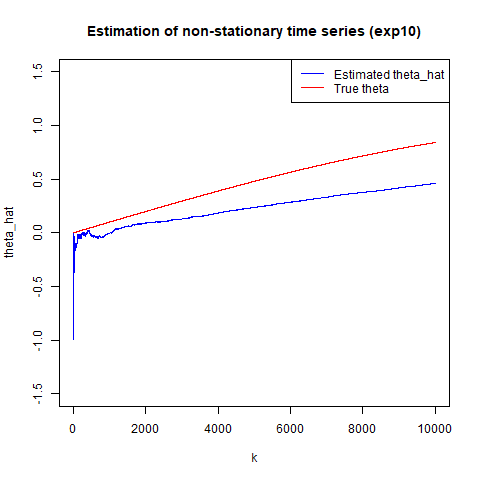
\includegraphics[width=.82\linewidth]{graphs/task10.png}
  \caption{忘却係数付きRLSによる非定常平均の追従($\gamma=0.99$)}
  \label{fig:task10}
\end{figure}

\paragraph{考察}
% 追従と平滑化のトレードオフ:$\gamma\downarrow$ で追従性↑ だが分散↑。$\gamma\uparrow$ で分散↓ だが遅延↑。
% 本設定は振幅1に対し雑音振幅1でSNRが低い。RMSEや相関係数で評価するとよい。
% スカラー回帰(φ_k=1)ではRLSは指数移動平均に近い挙動を示す。初期Φを大きくすると初期ゲインが大きく収束が速い。




% ===== 総合比較 =====
\section{アルゴリズム比較}
表や図を用いて複数手法の比較を行う。計算量・精度・安定性・実行時間の観点でまとめる。

\section{結論}
本章での結論と今後の課題を箇条書きでまとめる。

\appendix
\section{使用コード一覧}
主要スクリプトと入手先を列挙する。
\begin{itemize}
  \item 実験コード(R):\url{https://github.com/<your-repo>}
  \item データ生成スクリプト:\texttt{scripts/generate\_data.jl}
\end{itemize}

\section{補足導出}
必要な導出や補助的な数学的議論を載せる。

% ===== 参考文献 =====
\section*{参考文献}
\begin{thebibliography}{9}
\bibitem{exp2025} 数理工学実験(2025年度配布資料).
\end{thebibliography}

\end{document}
